%!TEX root = ../draft.tex
\chapter{Einleitung}\label{s.einleitung} 
In keinem Zeitabschnitt waren digitale Technologien so stark im Fokus wie heutzutage. Gerade der Bereich selbstständig lernender Computer wird in der Forschung untersucht und vorangetrieben. Auch bekannt unter dem Namen \textit{Deep Learning} oder künstliche Intelligenz (KI), ist mit diesen Bezeichnungen meist der Bereich der künstlichen neuronalen Netze gemeint. Solche Netze können durch eingeführte Datensätze oder Regeln lernen. Dadurch werden sie in dem trainierten Bereich \textit{intelligent}. Durch genügend Beispiele in den Trainingsdaten können sie Hypothesen aufstellen. Die Faktoren, welche beim Training wichtig sind, stellen zum einen die Menge, wie auch die Qualität der Trainingsdaten dar und zum anderen die Zeit in welcher das neuronale Netz trainiert wird. Mithilfe von steigender Rechenleistung kann das Verfahren beschleunigt werden, da normalerweise viel Zeit für das Training benötigt wird. In der Vergangenheit konnten die Forschungen aufgrund zu langsamer Hardware nicht effektiv weiter geführt werden. Mit der Leistung heutiger CPUs und GPUs ist dies ohne Probleme möglich.
\section{Problemstellung und Ziele}\label{s.probuziel} 
Beim Erstellen eines neuronalen Netzes können durch schlechte Trainigsdaten Schwierigkeiten entstehen. Im Bereich der Objekterkennung können dadurch Probleme, wie fehlerhafte Zuordnungen auftreten. Trainigsdaten bestehen üblicherweise aus mehreren Hunderttausend Bildern. Bei der Verwendung von vortrainierten Netzen reichen um die Tausend Bilder aus, um neue Klassen zu trainieren. Die richtige Ausleuchtung ist ein wichtiger Aspekt bei der Generierung von Trainingsbildern, da schon kleine Veränderungen der Lichtverhältnisse die Farben der Objekte verändern können. Ein und dasselbe Objekt kann dadurch in vielen verschiedenen Farbvariationen auftreten, wie man in Abbildung \ref{img:problem} erkennen kann. Durch weniger Licht wirken die Farben dunkler und unterscheiden sich sichtlich. Gerade bei einem Datensatz mit wenig Bildern, kann das zu fehlerhaften Prognosen führen. Häufig kann eine konstante Ausleuchtung nicht gewährleistet werden, weil die Bilder in der freien Umwelt erstellt werden und eine Ausleuchtung zu umständlich wäre. Das bedeutet, dass dieses Problem hauptsächlich in der Nachbereitung der Bilder angegangen werden kann.
\begin{figure}
	[h]
	\centering
	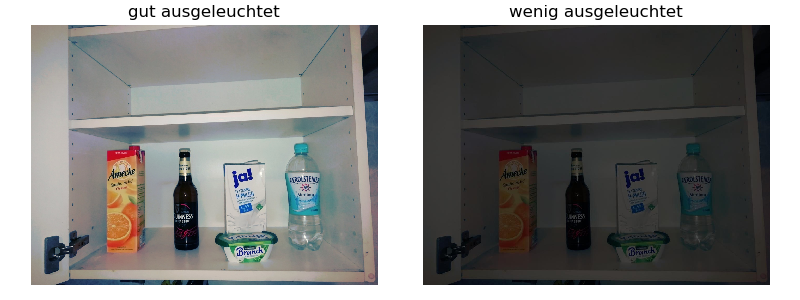
\includegraphics[scale=0.7]{Sources/Vergleich.png}
	\caption{Szene mit unterschiedlicher Ausleuchtung}
	\label{img:problem}
\end{figure}
\section{Erläuterung der These}\label{s.these}
Für solche Probleme bietet die Bildverarbeitung einige Lösungsansätze, welche theoretisch eine konstante Farbgebung und dadurch eine Erhöhung der Genauigkeit bringen könnten. Ob in der praktischen Ausführung die erwarteten Ergebnisse erzielt werden können, soll getestet werden. In dieser Arbeit sollen verschiedene Verfahren zur Farbnormalisierung von Bildern auf die Trainings- und Testdatensätze angewendet werden. Mit diesen normalisierten Datensätzen sollen daraufhin verschiedene künstliche neuronale Netze trainiert werden. Beim Vergleich der Trainingsergebnisse soll herausgestellt werden, ob das Normalisieren der Daten einen positiven Einfluss auf die Genauigkeit hat und welche Unterschiede die Normalisierungs-Verfahren aufweisen.
\section{Anforderungen}\label{s.anforderungen}
Bei dem geplanten Vorhaben, welches diese Arbeit thematisiert, ist es wichtig Anforderungen an das neuronale Netz, den Datensatz und die verwendeten Algorithmen zu formulieren, um sicher zu stellen, dass keine vermeidbaren Probleme auftreten. Zunächst werden Trainingsdaten benötigt, mit welchen die neuronalen Netze trainiert werden. Viele wissenschaftliche Arbeiten zeigen, dass eine große Menge an Daten benötigt wird, um ein gut funktionierendes neuronales Netz zu entwickeln. Im Schnitt werden 50.000 Trainingsbilder pro Klasse benötigt. Diese Menge an Daten kann in Anbetracht der verfügbaren Zeit nicht für drei verschiedene Datensätze generiert werden. Da die benötigten Ressourcen nicht zur Verfügung stehen, soll eine Möglichkeit gefunden werden, gute Ergebnisse mit einer geringeren Menge an Trainingsdaten zu realisieren. Damit genügend Vergleichswerte untersucht werden können, sollen mehrere Datensätze mit unterschiedlichen Klassen genutzt werden. Um sicher zu stellen, dass die Datensätze für das Vorhaben geeignet sind, werden diese für die Arbeit erstellt und ausgesucht.\\\\
Die Trainingsdaten sollen unter folgenden Anforderungen erstellt werden:
\begin{enumerate} 
\item Ein qualitativ hochwertiger Datensatz sollte nicht unordentlich sein, da das Reinigen der Daten lange dauern kann. Das bedeutet, dass Klassen getrennt voneinander gespeichert werden, und die Namensgebung für jede Objektklasse klar definiert ist. Bei Problemfällen können Daten entfernt oder hinzugefügt werden.
\item Der Datensatz sollte Bilder enthalten, welche eine nicht zu hohe Auflösung besitzen, da sie den Trainingsfortschritt zurückhalten und mehr Ressourcen benötigen. Je größer das Bild ist, desto mehr Zeit wird für die Verarbeitung benötigt.
\item Beim Generieren der Trainingsbilder sollte darauf geachtet werden, saubere und gut ausgeleuchtete Aufnahmen zu machen. Aufnahmen der Objekte sollten nicht zu stark verschwimmen und unscharf werden. 
\item Das Ziel des Datensatzes sollte gut definiert werden. Namen und Thema des Datensatzes sollten auf einen gewissen Bereich beschränkt werden (zum Beispiel: keine Gesichter zusammen mit Pflanzen kombinieren). 
\end{enumerate}
Um die Auswirkungen der Normalisierungsverfahren vergleichen zu können werden verschiedene Verfahren auf die selben Trainings- und Testdaten angewendet. Durch die Normalisierungsverfahren soll die Farbvarianz verringert werden.
  \section{Struktur der Arbeit}\label{Struktur} 
Für ein besseres Verständnis der einzelnen Entwicklungsschritte in den späteren Kapiteln werden in Kapitel \ref{s.digibilder} zuerst die Grundlagen der digitalen Bildverarbeitung beschrieben. Dabei soll zunächst vermittelt werden wie digitale Bilder entstehen und aus welchen Komponenten diese zusammengesetzt sind. Im Weiteren wird in Kapitel \ref{s.neuronalenetze} auf die Funktionsweise künstlicher neuronaler Netze eingegangen. Hierbei werden die unterschiedlichen Schichten welche durchlaufen werden aufgeführt und beschrieben. Anschließend werden in Kapitel \ref{s.nalgorithmen} die verwendeten Farbnormalisierungsverfahren erklärt und beschrieben. Der Ansatz der einzelnen Methoden wird erläutert, sowie die verwendeten Trainingsdaten und Modelle.\\\\
In der zweiten Hälfte der Arbeit wird es um die Durchführung und Ergebnisauswertung (Kapitel \ref{s.ergebnisse}) des praktischen Teils der Arbeit gehen. In diesem werden die verwendeten Farbnormalisierungsverfahren zusätzlich in der technischen Umsetzung erläutert. Daraufhin werden die Ergebnisse und interpretiert. In einer kurzen Diskussion (Kapitel \ref{s.diskussion}) werden diese behandelt. Nach der Diskussion wird nun das Ergebnis der Auswertung anhand der angeführten These evaluiert und ein Fazit (Kapitel \ref{s.fazit}) der Arbeit getroffen.